\chapter*{Задание №3}
Задание: потомки переходят на выполнение других программ, которые передаются системному вызову exec() в качестве параметра. Потомки должны выполнять разные программы. Предок ждет завершения своих потомков с анализом кодов завершения. На экран выводятся соответствующие сообщения.

В данном задании системному вызову exec() были переданы исполняемые файлы "main\_1.out" и "main\_2.out". Программа main\_1.out соответствует программной реализации алгоритма полиномиальной интерполяции табличных функций. Программа main\_2.out соответствует программной реализации алгоритма сплайн-интерполяции табличных функций.

\begin{lstlisting}[label = exec, caption=Использование системного вызова exec().]
#include <unistd.h>
#include <stdio.h>
#include <sys/wait.h>

#define FORK_ERROR -1
#define FORK_OK 0

#define COUNT_CHILDS 2

int main(void)
{
	pid_t childs_pid[COUNT_CHILDS];
	pid_t child_pid;
	
	char *command_args[COUNT_CHILDS] = {"/home/lev/workspace/lab_04_os/main_1.out", "/home/lev/workspace/lab_04_os/main_2.out"};
	
	int res_exec = 0;
	
	printf("Parent - pid: %d, pgrp: %d\n", getpid(), getpgrp());
	
	for (int i = 0; i < COUNT_CHILDS; i++)
	{
		child_pid = fork();
		if (child_pid == FORK_ERROR)
		{
			perror("Can't fork.\n");
			return 1;
		}
		else if (child_pid == FORK_OK)
		{
			printf("Child - pid: %d, ppid: %d, pgrp: %d\n", getpid(), getppid(), getpgrp());
			if (i == 0){
				res_exec = execlp(command_args[i], "main_1.out", "table_1_newton.txt",
				                  (char *)NULL);
			}
			else{
				res_exec = execlp(command_args[i], command_args[i], (char *)NULL);
			}
			
			if (res_exec == -1){
				perror("Can't child exec(). ");
			}
			return 0;
		}
		else{
			childs_pid[i] = child_pid;
		}
		
	}
	
	for (int i = 0; i < COUNT_CHILDS; i++)
	{
		int status;
		pid_t child_pid;
		child_pid = wait(&status);
		
		printf("Child has finished - pid: %d, ppid = %d\n", child_pid, getppid());
		
		if (WIFEXITED(status)){
			printf("Child exited with code %d\n", WEXITSTATUS(status));
		}
		else {
			printf("Child terminated abnormally.\n");
		}
	}    
	
	printf("Parent-child_1_pid: %d, child_2_pid: %d, child_3_pid: %d\n",
	       childs_pid[0], childs_pid[1], childs_pid[2]);
	printf("Parent process is dead\n");
	
	return 0;
}
\end{lstlisting}


Результат работы программы представлен на рисунке \ref{png:res_3}:

\begin{figure}[H]
	\centering{
		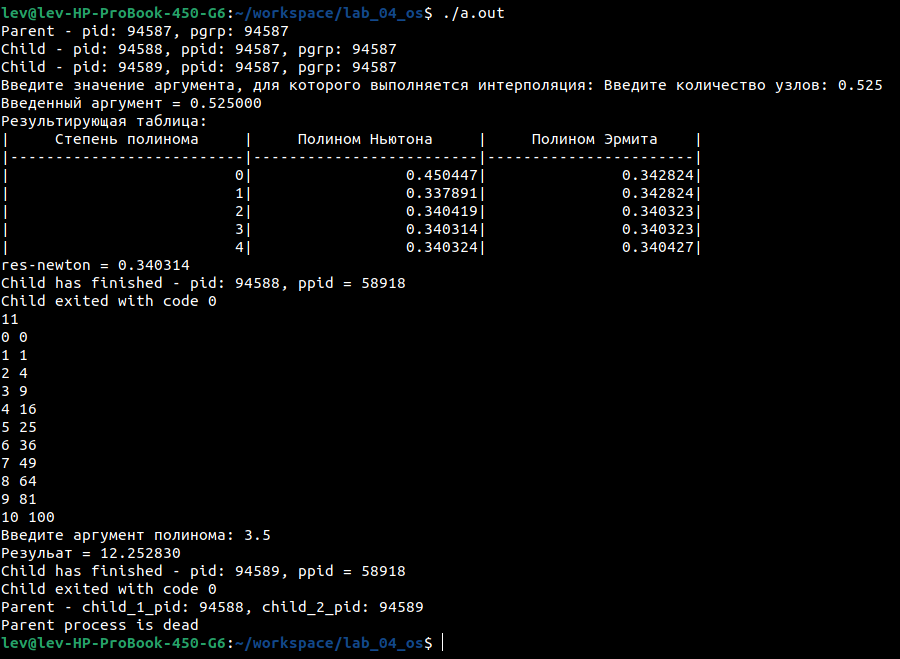
\includegraphics[scale=0.5]{../../../../../../../msys64/home/Лев/bmstu_sem_5_os/lab_04/report/images/task_3}
		\caption{Демонстрация работы программы (задание 3).}
		\label{png:res_3}}
\end{figure}